%
% riemann.tex
%
% (c) 2020 Prof Dr Andreas Müller, Hochschule Rapperswil
%
\section{Riemann-Integral und Trapezregel
\label{buch:section:integraldefinition}}
\rhead{Riemann-Integral und Trapezregel}
Die Stammfunktion 
\[
F(x) =  \int_a^x f(t)\,dt
\]
einer Funktion $f(x)$ ist die Lösung der besonders einfachen
Differentialgleichung $y'=f(x)$, man könnte also dieses Kapitel
einfach überspringen und für die Berechnung von Integralen auf
die Methoden zur Lösung gewöhnlicher Differentialgleichungen
verweisen.
Dies ist aber nicht unbedingt sinnvoll.
Das bestimmte Integral einer Funktion zwischen zwei
Grenzen ist ein wesentlich einfacheres Konzept als die Lösung einer
Differentialgleichung, man darf daher davon ausgehen, dass es
auch einfachere Berechnungsverfahren dafür geben dürfte.
Die relativ komplizierten Lösungsverfahren für gewöhnliche
Differentialgleichungen dürften viel zu viel rechnen für das gestellte Problem.

Wir erwarten daher, dass spezialisierte Verfahren zur Berechnung von
Integralen folgende Eigeschaften haben:
\begin{enumerate}
\item Einfache Anwendung: Der Code zur Berechnung eines Integrals
sollte sehr viel einfacher ausfallen als der Code zur Lösung einer
Differentialgleichung.
\item Allgemein anwendbar: Das Verfahren sollte für eine grosse Klasse
von Integranden anwendbar sein, auch für solche, für die Lösungsverfahren
für gewöhnliche Differentialgleichungen schwierig zu konstruieren sind.
Zum Beispiel verlangen die Eindeutigkeitssätze für gewöhnliche
Differentialgleichungen typischerweise eine Lifshitz-Eigenschaft.
Integrale sollten aber auch von Funktionen berechnet werden können, die
eine solche Eigenschaft nicht haben.
\item Schnelle Konvergenz für ``gute'' Integranden.
Glatte Integranden sollten nur an wenigen Stellen ausgewertet werden müssen
und bereits gute Resultate ergeben.
\end{enumerate}
Der besser geeignete Ausgangspunkt für die Konstruktion eines 
Integrationsverfahrens ist daer die usrprüngliche Definition des
Riemann-Integrals, welche wir in Abschnitt~\ref{buch:subsection:riemann}
rekapitulieren.
Daraus ergibt sich dann die Mittelpunktsformel in
Abschnitt~\ref{buch:subsection:mittelpunkt}, deren Fehlerverhalten in
Abschnitt~\ref{buch:subsection:mittelfehler} untersucht wird.

\subsection{Das Riemann-Integral
\label{buch:subsection:riemann}}
\begin{figure}
\centering
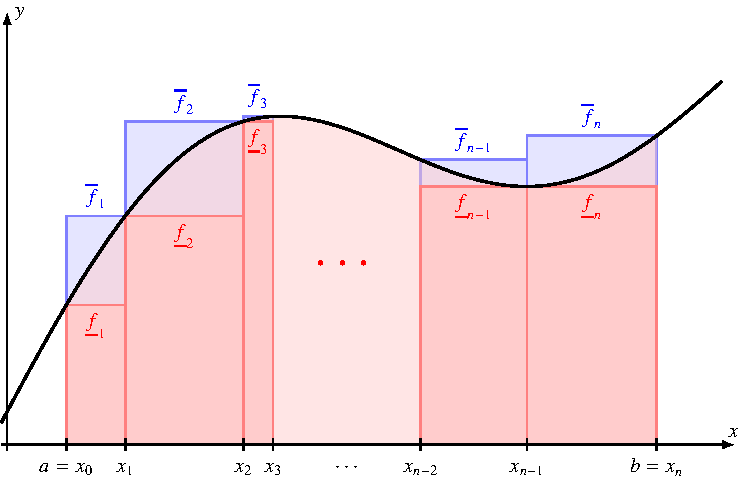
\includegraphics{chapters/40-integration/figures/riemann.pdf}
\caption{Definition der oberen und unteren Riemann-Summe und des
Riemann-Integrals
\label{buch:figure:riemann}}
\end{figure}
Im Analysisunterricht wird das Riemann-Integral
\begin{equation}
I = \int_a^b f(x)\,dx
\label{buch:integral}
\end{equation}
einer Funktion $f(x)$ zwischen den Grenzen $a$ und $b$ üblicherweise
wie folgt definiert.
Zunächst wird das Interval $[a,b]$ mit Hilfe einer Menge
$D=\{x_0,x_1,x_2,\dots,x_{n-1}, x_n\}$
von Zwischenpunkten mit der Eigenschaft
\[
a=x_0 < x_1 < x_2 < \dots < x_{n-1} < x_n = b
\]
unterteilt.
Das {\em Korn} der Unterteilung ist die Länge des längsten Teilintervals
\[
\delta(D) = \max_{0\le i< n} |x_{i+1}-x_i|.
\]
Als Approximationen des Integrals~\eqref{buch:integral} werden dann die
obere und untere Riemann-Summe
\begin{align*}
\overline{I}(D)
&=
\sum_{i=1}^n \overline{f}_i (x_i-x_{i-1})
&&\text{mit}
&\overline{f}_i
&=
\max_{\xi\in [x_{i-1},x_i]} f(\xi)
\\
\underline{I}(D)
&=
\sum_{i=1}^n \underline{f}_i (x_i-x_{i-1})
&&\text{mit}
&\underline{f}_i
&=
\min_{\xi\in [x_{i-1},x_i]} f(\xi)
\end{align*}
gebildet.
Aufgrund der Konstruktion ist klar, dass $\underline{I} \le I \le \overline{I}$
sein muss.
Für einigermassen ``glatte'' Funtionen wird der Unterschied zwischen
$\overline{I}(D)$ und $\underline{I}(D)$ kleiner werden, wenn man die 
Unterteilung verfeinert.
Falls die obere und die untere Riemann-Summe bei Verfeinerung gegen
den gleichen Grenzwert streben, sagt man, das {\em Riemann-Integral}
\index{Riemann-Integral}%
existiere und habe den Wert
\[
I
=
\int_a^b
=
\lim_{\delta(D)\to 0} \underline{I}(D)
=
\lim_{\delta(D)\to 0} \overline{I}(D).
\]
Wenn das Integral existert, kann man offenbar auch jeden beliebigen
anderen anderen Wert der Funktion in den Teilintervallen $[x_{i-1},x_i]$
verwenden.
Eine Summe der Form
\[
\sum_{i=1}^n f(\xi_i) (x_{i}-x_{i-1})
\qquad\text{mit}\qquad \xi_i \in [x_{i-1},x_i],
\]
auch {\em Riemann-Summe} genannt,
ist für jede beliebige Wahl der Unterteilung $D$ und der Zwischenpunkte
$\xi_i$ ein Approximation des Integrals $I$ von \eqref{buch:integral}.

Die Riemann-Summe liefert also bereits eine direkte Berechnungsmöglichkeit
für ein beliebiges Integral, und sie liefert uns auch bereits ein Möglichkeit,
die Grössenordnung des zu erwartenden Fehlers abzuschätzen:
Die Differenz $\overline{I}(D)-\underline{I}(D)$ ist der grösste mögliche
Fehler.
Der Berechnungsaufwand lässt sich ebenfalls sehr gut abschätzen.
Es muss eine Summe von $n$ Termen gebildet werden, in jeder Summe
wird eine Differenz aufeinanderfolgender Teilpunkte gebildet und
ein Produkt mit dem Funktionswert.
Es wird offensichtlich, dass ausser für sehr einfache Funktionen, für die
man das Integral auch analytisch ausrechnen könnte, der Hauptteil der
Arbeit in der Berechnung der Funktionswert $f(\xi_i)$ steckt.

Die Riemann-Summe beinhaltet einige Wahlmöglichkeiten, mit der die
Berechnung optimiert werden kann.
Wir können die Teilpunkte $D$ wählen und zum Beispiel die Unterteilung
dort feiner wählen, wo die Funktion sich schnell verändert.
Wir können auch die Zwischenpunkte wählen.
Für beides ist jedoch eine detaillierte Kenntnis der Funktion notwendig,
welche nur durch die Berechnung zusätzlicher Funktionswerte gewonnen
werden kann.

\subsection{Mittelpunktsregel
\label{buch:subsection:mittelpunkt}}
\begin{figure}
\centering
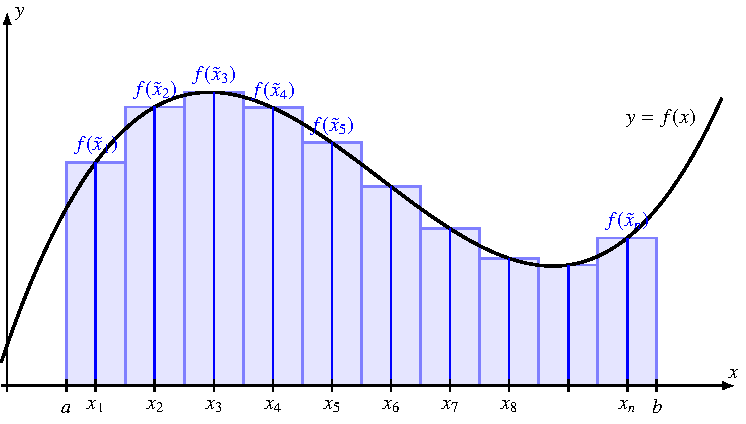
\includegraphics{chapters/40-integration/figures/mittelpunkt.pdf}
\caption{Approximation eines Integrals mit Hilfe der Mittelpunktsregel
\label{buch:figure:mittelpunkt}}
\end{figure}
Die einfachste Art der Unterteilung des Intervalls ist Teilinterval
konstanter Länge zu verwenden. 
Wir schreiben
\[
h = \frac{b-a}n
\qquad\text{und}\qquad
x_i = a + ih
\]
für die Intervalllänge und die Teilpunkte.
Werten wir die Funktion im Mittelpunkt eines Teilintervals aus, also
in $\xi = (x_{i-1}+x_i)/2 = x_{i-1}+\frac12h = x_i -\frac12h$,
erhalten wir als Approximation für das Integral~\eqref{buch:integral}
die {\em Mittelpunktsregel}
\begin{equation}
M(h)
=
\sum_{i=1}^n f\biggl(x_i - \frac{h}2\biggr) \cdot h
=
h
\sum_{i=1}^n f\bigl(a+(i-{\textstyle\frac12})h\bigr).
\label{buch:equation:mittelpunktsregel}
\end{equation}
Die Approximation wird in Abbildung~\ref{buch:figure:mittelpunkt}
veranschaulicht.
Für die Berechnung der Summe~\eqref{buch:equation:mittelpunktsregel}
sind genau $n$ Auswertungen der Funktion $f(x)$ notwendig.

\begin{beispiel}
\label{buch:beispiel:kreis}
Als Beispiel approximieren wir das Integral
\[
I
=
\int_{1}^{9} x\,dx
=
\left[\frac{x^2}2\right]_1^9
=
\frac{9^2-1^2}2=\frac{81-1}2=40
\]
mit Schritten der Schrittweite $h=2$.
Die Zwischenpunkte sind $x_1=2$, $x_2=4$, $x_3=6$, $x_4=8$ oder $x_n=2n$.
Die Mittelpunktregel liefert die Approximation
\[
M(2)
=
\sum_{i=1}^n f(2i) \cdot 2
=
\sum_{i=1}^n 4i
=
4\sum_{i=1}^n i
=
4\cdot \frac{n(n+1)}{2}
=
4\cdot\frac{4\cdot 5}{2}
=
4\cdot 2 \cdot 5
=
40.
\]
In diesem Beispiel liefert die Mittelpunktformel also den exakten Wert
des Integrals.
Grund dafür ist natürlich, dass der Graph eine Gerade ist, und die 
``fehlenden'' Dreieck in der Summe $M(h)$ links und rechts vom
Funktionswert genau gleich gross sind, sich diese Fehler also wegheben.
\end{beispiel}
Das Beispiel illustriert, dass die Approximation gar nicht so schlecht ist,
wie sich auf Grund der deutlich hervortretenden Stufen in
Abbildung~\ref{buch:figure:mittelpunkt} vielleicht vermuten lässt.


\subsection{Trapezregel
\label{buch:subsection:trapez}}
\begin{figure}
\centering
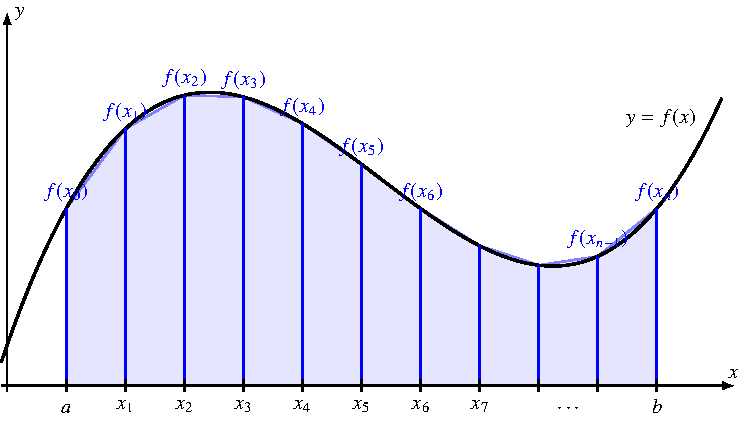
\includegraphics{chapters/40-integration/figures/trapez.pdf}
\caption{Approximation eines Integrals mit Hilfe der Trapezregel
\label{buch:figure:trapez}}
\end{figure}
Statt die Fläche unter dem Graphen von $f(x)$ in jedem Teilinterval
durch den Wert im Mittelpunkt des Intervalls zu berechnen wie bei der
Mittelpunktsregel, könnte sie auch approximiert werden durch ein
Trapez mit Eckpunkten $(x_{i-1},0)$, $(x_i,0)$,
$(x_{i-1},f(x_{i-1}))$ und
$(x_i,f(x_i))$.
Die Mittellinie eines solchen Trapezes hat die Länge
$\frac12(f(x_{i-1}) +f(x_i))$, die Höhe ist $h$.
Der Flächeninhalt eines einzelnen Trapezes ist daher
$\frac{h}2(f_(x_{i-1}+f(x_i))$ und es ergibt sich die Approximation
\begin{align}
\int_a^b
f(x)\,dx
&\simeq
T(h)
=
\frac{h}2
\sum_{i=1}^n \bigl(f(x_{i-1} + f(x_i)\bigr)
\notag
\\
&=
\bigl(
{\textstyle\frac12}f(x_0) + f(x_1) + f(x_2)
+ \dots
+ f(x_{n-2}) + f(x_{n-1}) + {\textstyle\frac12} f(x_n)
\bigr)\cdot h
\label{buch:equation:trapez}
\end{align}
für das Integral.
In Abbildung~\ref{buch:figure:trapez} ist die Summe der Trapezflächen 
dargestellt.
Die Approximation $T(h)$ in \eqref{buch:equation:trapez} heisst
{\em Trapezregel}.
\index{Trapezregel}%
Die Trapezregel erfordert genau $n+1$ Funktionsauswertungen.

\subsubsection{Verfeinerung}
Die Trapezregel $T(h)$ benötigt die Funktionswerte an den Stellen $x_i=a+hi$.
Halbiert man die Schrittweite, müssen zusätzlich die Funktionswerte
an den Zwischenpunkten
\[
\frac{x_{i-1}+x_{i}}{2}
= 
a+h(i-{\textstyle\frac12})
\]
für $i=1,\dots,n$ bestimmt werden.
Das sind genau die Funktionswerte, die in der Mittelpunktformel
summiert wurden.
Somit kann man die Trapezsumme $T(\frac{h}2)$ durch Umordnen der Terme
in der Summe durch die Trapezsummen $T(h)$ und die Mittelpunktformel
$M(h)$ ausdrücken:
\begin{align}
T({\textstyle\frac{h}2})
&=
\frac{h}2\cdot
\bigl(
{\textstyle\frac12}
f(a)
+
f(a+1\cdot {\textstyle\frac{h}2})
+
f(a+2\cdot {\textstyle\frac{h}2})
+
\dots
f(a+(2n-1)\cdot {\textstyle\frac{h}2})
+
{\textstyle\frac12}
f(a+2n\cdot {\textstyle\frac{h}2})
\bigr)
\notag
\\
&=
\frac{h}2\cdot
(\text{gerade Terme})
+
\frac{h}2\cdot
(\text{ungerade Terme})
\notag
\\
&=
\frac{h}2 \left(
{\textstyle\frac12}
f(a)
+
f(a+2\cdot {\textstyle\frac{h}2})
+
f(a+4\cdot {\textstyle\frac{h}2})
+
\dots
+
{\textstyle\frac12}
f(a+(2n)\cdot {\textstyle\frac{h}2})
\right)
\notag
\\
&\qquad
+
\frac{h}2 \left(
f(a+1\cdot {\textstyle\frac{h}2})
+
f(a+3\cdot {\textstyle\frac{h}2})
+
\dots
+
f(a+(2n-1)\cdot {\textstyle\frac{h}2})
\right)
\notag
\\
&=
\frac12\cdot h\cdot
\left(
{\textstyle\frac12}
f(a)
+
f(a+h)
+
f(a+2h)
+
\dots
+
{\textstyle\frac12}
f(a+nh)
\right)
\notag
\\
&\qquad
+
\frac12 \cdot h\cdot \left(
f(a+(1-{\textstyle\frac12})h)
+
f(a+(2-{\textstyle\frac12})h)
+
\dots
+
f(a+(n-{\textstyle\frac12})h)
\right)
\notag
\\
&=
\frac12 T(h) 
+
\frac12 M(h).
\label{buch:equation:TMrekursion}
\end{align}
Halbierung der Schrittweite bedeutet daher nur, dass man die
Mittelpunktregel $M(h)$ zusätzlich auswerten muss.

Für die Berechnung von $T(\frac{h}2)$ sind $2n+1$ Funktionsauswertungen
notwendig, davon entfallen $n+1$ auf die Berechnung von $T(h)$ und
$n$ auf die Berechnung von $M(h)$.

\begin{beispiel}
Als Beispiel berechnen wir das Integral 
\begin{equation}
I
=
\int_0^1 \sqrt{1-x^2}\,dx.
\label{buch:equation:kreis}
\end{equation}
Es berechnet die Fläche des im ersten Quadranten liegenden Teils des
Einheitskreises, hat also den Wert $I=\frac{\pi}4\simeq 0.78539816$.

Das folgende Octave-Programm kann zur Berechnung verwendet werden:
\lstinputlisting[language=Octave,style=Octave]{chapters/40-integration/trapez.m}
In Zeile~5 wird der Integrand als Funktion definiert.
In Zeile~9 wird die Funktion \texttt{M(h,a,b,f)} definiert, die
die Mittelpunktsumme $M(h)$ der Funktion $f$ berechnet.
Es ist nicht nötig, eine Funktion für $T(h)$ zu definieren, da
sich der Wert $T({\textstyle\frac{h}2})$ aus $T(h)$ und $M(h)$ ergibt.
In Zeile~19 wird der erste Wert $T(1)$ berechnet,
In der nachfolgenden Schleife zwischen Zeilen 21 und 24 wird die
Rekursion \eqref{buch:equation:TMrekursion} angewendet.
Die sich ergebenden Zahlenwerte sind in Tabelle~\ref{buch:table:kreis}
zusammengestellt.

\begin{table}
\centering
\renewcommand\arraystretch{1.15}
\begin{tabular}{|>{$}c<{$}|>{$}c<{$}|>{$}c<{$}|}
\hline
   k& T(h)                           & h                  \\
\hline
   1&  0.\underline{}5000000000000000&  1.0000000000000000\\
   2&  0.\underline{}6830127018922193&  0.5000000000000000\\
   3&  0.\underline{7}489272670256102&  0.2500000000000000\\
   4&  0.\underline{7}724547860892934&  0.1250000000000000\\
   5&  0.\underline{78}08132594569352&  0.0625000000000000\\
   6&  0.\underline{78}37756057192828&  0.0312500000000000\\
   7&  0.\underline{78}48242281949210&  0.0156250000000000\\
   8&  0.\underline{785}1951980991537&  0.0078125000000000\\
   9&  0.\underline{7853}263957393075&  0.0039062500000000\\
  10&  0.\underline{7853}727881799138&  0.0019531250000000\\
  11&  0.\underline{7853}891916347545&  0.0009765625000000\\
  12&  0.\underline{78539}49913528619&  0.0004882812500000\\
  13&  0.\underline{78539}70419019385&  0.0002441406250000\\
  14&  0.\underline{78539}77668874246&  0.0001220703125000\\
  15&  0.\underline{785398}0232097235&  0.0000610351562500\\
  16&  0.\underline{7853981}138335553&  0.0000305175781250\\
  17&  0.\underline{7853981}458739578&  0.0000152587890625\\
  18&  0.\underline{7853981}572019572&  0.0000076293945312\\
  19&  0.\underline{78539816}12070116&  0.0000038146972656\\
  20&  0.\underline{78539816}26230124&  0.0000019073486328\\
\hline
    &  0.7853981633974483            &                    \\
\hline
\end{tabular}
\caption{Approximation des Integrals~\eqref{buch:equation:kreis}
mit Hilfe der Trapezregel.
Unterstrichen die Stellen des Wertes von $T(h)$, die bereits korrekt sind.
\label{buch:table:kreis}}
\end{table}
Für den Wert von $T(h)$ in Zeile $k$ der Tabelle sind
$2^{k-1}+1$ Funktionsauswertungen nötig,
auf der letzen Zeile sind dies 524289 Funktionsauswertungen.
Es fällt auf, dass die Konvergenz ziemlich langsam ist.
Der Fehler von $T(h)$ nimmt ungefähr so schnell ab, wie $h$ kleiner wird.
Sollte sich diese Systematik bestätigen lassen, könnte man daraus ein
Verfahren zur Beschleunigung der Konvergenz ableiten.
\end{beispiel}

\subsection{Fehler von Trapez- und Mittelpunktsregel
\label{buch:subsection:mittelfehler}}
Im Beispiel im vorangenangenen Abschnitt hat sich in
Tabelle~\ref{buch:table:kreis} eine Gesetzmässigkeit in Entwicklung der
Fehler von $T(h)$ gezeigt.
Es schien, als wäre $I-T(h)\sim h$.
Ziel dieses Abschnittes ist, dies nachzuweisen.
Als Werkzeug dafür benötigen wir die Euler-Maclaurinsche Summenformel.


\subsubsection{Partielle Integration}
Der Fehler der Trapezregel dürfte umso grösser werden, je stärker der
Graph der Funktion $f(x)$ gekrümmt ist.
Wir vermuten daher einen Zusammenhang zwischen dem Fehler und der
zweiten Ableitung von $f(x)$.
Um diesen Zusammenhang zu finden, betrachten wir das Integral
\begin{equation}
I = \int_0^1 g(t) \,dt.
\label{buch:equation:basispartint}
\end{equation}
Den Integranden können wir auch als Produkt $1\cdot g(t)$ der
konstanten Funktion $1$ mit $g(t)$ schreiben und das Integral
partiell ausführen:
\begin{align}
I
&=
\int_0^1 1\cdot g(t)\,dt
=
\biggl[ p_1(t) \cdot g(t) \biggr ]_0^1 
- 
\int_0^1 p_1(t)\cdot g'(t) \,dt
\notag
\intertext{wobei wir für $p_1(t)$ ein beleibiges Polynom wählen können,
dessen Ableitung $p_1'(t)=1$ ist.
Das zweite Integral können wir nochmals partiell integrieren und
erhalten
}
&=
\biggl[ p_1(t) \cdot g(t) \biggr ]_0^1 
- 
\biggl[ p_2(t)\cdot g'(t) \biggr]_0^1
+
\int_0^1 p_2(t)\cdot g''(t) \,dt
\notag
\intertext{wobei wieder $p_2'(t)=p_1(t)$ sein muss.
Dieser Prozess lässt sich natürlich wiederholen und ergibt nach $k$
Schritten
}
&=
\biggl[ p_1(t) \cdot g(t) \biggr ]_0^1 
- 
\biggl[ p_2(t)\cdot g'(t) \biggr]_0^1
+
\biggl[ p_3(t) \cdot g''(t) \biggr ]_0^1 
-
\biggl[ p_4(t)\cdot g'''(t) \biggr]_0^1
+
\dots
\notag
\\
&
\qquad
-
(-1)^k
\biggl[ p_k(t)\cdot g^{(k-1)}(t) \biggr]_0^1
+
(-1)^k
\int_0^1 p_k(t) g^{(k)}(t)\,dt
\label{buch:equation:partintsumme}
\end{align}
Die Polynome $p_k(t)$ sind bis jetzt noch nicht eindeutig festgelegt, es ist
nur die Rekursionsformel
\[
p'_k(t) = p_{k-1}(t)
\qquad\text{für alle $k>0$ und}\qquad
p_0(t) = 1
\]
gegeben.
Durch eine geschickte Wahl der Polynome soll jetzt aus der Entwicklung
möglichst viel Information über das Integral extrahiert werden.

Wir betrachten zunächst den Fall, dass $g(t)$ selbst ein Polynom ist.
Genügend hohe Ableitungen eines Polynoms verschwinden, ist die Ordnung $k$
der Ableitung grösser als der Grad des Polynoms, dann ist $g^{(k)}(t)=0$.
Dies bedeutet, dass in der Summe~\eqref{buch:equation:partintsumme}
der Integralterm verschwindet, sobald $k$ grösser als der Grad von $g$ ist.
Aber auch für $k=\deg g$ kann man den letzten Term zum verschwinden
bringen, wenn man $p_k(t)$ geeignet wählt.
In diesem Fall ist $g^{(k)}(t)$ konstant, der Integralterm verschwindet
also genau dann, wenn das Integral von $p_k(t)$ verschwindet.
Wir legen daher die Polynome $p_k(t)$ durch die Forderung fest, dass
\begin{equation}
\int_0^1 p_k(t)\,dt = 0\qquad\forall k
\end{equation}
sein soll.

\subsubsection{Die Polynome $p_k(t)$}
Wir berechnen die ersten paar Polynome der Folge $p_k(t)$.
Zunächst ist $p_1(t) = t+C$, wir müssen also $C$ so wählen, dass
das Integral
\[
\int_0^1 p_1(t)\,dt
=
\int_0^1 t+C\,dt
=
\biggl[\frac12t^2 + Ct\biggr]_0^1
=
\frac12 + C
\]
verschwindet.
Es folgt $C=-\frac12$ und $p_1(t)=t-\frac12$.

Für $p_2(t)$ folgt zunächst durch Integration $p_2(t)=\frac12t^2-\frac12t+C$
und dann aus der Integralbedingung
\[
\int_0^1 p_2(t) \,dt
=
\biggl[
\frac16t^3-\frac14t^2+Ct
\biggr]_0^1
=
\frac16-\frac14+C
=
-\frac1{12}+C,
\]
woraus $C=\frac1{12}$ folgt und damit
$p_2(t) = \frac12t^2 -\frac12t-\frac1{12}$.
Auf dies Art kann man schrittweise die folgenden Polynome finden:
\begin{align*}
p_1(t)
&=
t-\frac12
\\
p_2(t)
&=
\frac12t^2 - \frac12t +\frac1{12}
\\
p_3(t)
&= 
\frac16t^3 - \frac14t^2 +\frac1{12}t
\\
p_4(t)
&=
\frac1{24}t^4-\frac12t^3 + \frac1{24} t^2 - \frac1{720}
\\
p_5(t)
&=
\frac1{120}t^5 - \frac{1}{240} t^4+\frac1{360} t^3 -\frac1{3600}t
\end{align*}
Der führende Koeffizient des Polynoms $p_k(t)$ ist $1/k!$, indem man
diesen ausklammert, kann man etwas einfachere Polynome bekommen:
\begin{align*}
       &                         & B_0(t) &= 1                                \\
p_1(t) &= 1         \cdot B_1(t) & B_1(t) &= t -\frac12                       \\
p_2(t) &= \frac1{2!}\cdot B_2(t) & B_2(t) &= t^2 - t + \frac16                \\
p_3(t) &= \frac1{3!}\cdot B_3(t) & B_3(t) &= t^3-\frac32 t^2+\frac12t         \\
p_4(t) &= \frac1{4!}\cdot B_4(t) & B_4(t) &= t^4-2t^3+t^2-\frac1{30}          \\
p_5(t) &= \frac1{5!}\cdot B_5(t) & B_5(t) &= t^5-\frac52t^4-\frac53t^3-\frac16t
\end{align*}
Die Polynome $B_k(t)$ heissen {\em Bernoulli-Polynome}.
\index{Bernoulli-Polynome}

\subsubsection{Eigenschaften der Polynome $p_k(t)$}
Auch ohne die expliziten Formeln des vorangenangen Abschnittes lassen sich
nützliche Symmetrieeigenschaften der Polynome $p_k(t)$ bezüglich des
Punktes $t=\frac12$ ableiten.

Die Symmetrieeigenschaften sind etwas verschleiert durch die Wahl
des Intervals $[0,1]$ als Definitionsbereich.
Wir untersuchen die Symmetrie der Polynome bezüglich des Punktes
$t_0=\frac12$.
Wir schreiben $\tilde{p}_k(t)$ für die Stammfunktion von $p_{k-1}(t)$ 
mit Integrationskonstante $C_k=0$, es ist also
\[
p_k(t) = \tilde{p}_k(t) + C_k
\qquad\text{und}\qquad
\tilde{p}_k(0)=0.
\]
Die Integrationskonstante $C_k$ wurde im vorangegangenen Abschnitt
jeweils bestimmt.

Zunächst halten wir fest, dass die Polynome $p_k(t)$ alle
entweder gerade oder ungerade sind bezüglich $t_0$.

\begin{lemma}
\label{buch:lemma:pk}
Die Polynome $p_{2k}(t)$ sind gerade bezüglich $t_0$, die Polynome
$p_{2k+1}(t)$ sind ungerade bezüglich $t_0$.
Insbesondere ist $p_{2k}(t)(0)=p_{2k}(1)$ und
$p_{2k+1}(1)=-p_{2k+1}(0)$.
\end{lemma}

\begin{proof}[Beweis]
Die ersten zwei Polynome $p_0(t)=1$ und $p_1(t)=t-\frac12$ haben
tatsächlich die genannten Symmetrieeigenschaften.
Um die Aussage zu beweisen muss jetzt also nur untersucht werden,
dass $p_k(t)$ die verlangten Eigenschaften hat, wenn alle vorangegangenen
Polynome die ``richtigen'' Symmetrien hat.

Nehmen wir an, dass $p_{k-1}(t)$ gerade ist bezüglich $t_0$,
wir müssen zeigen, dass $p_k(t)$ ungerade bezüglich $t_0$ ist.
Zunächst ist klar, dass $p_k(t)-p_k(t_0)$ ungerade ist bezüglich
$t_0$.
Folglich verschwindet das Integral von $p_k(t)-p_k(t_0)$ oder
\[
0
=
\int_0^1p_{k}(t)-p_{k}(t_0)\,dt
=
\int_0^1p_k(t)\,dt - p_k(t_0)
=
-p_k(t_0),
\]
d.~h.~auch $p_k(t_0)$ verschwindet und $p_k(t)$ ist bereits ungerade
bezüglicch $t_0$.

Nehmen wir jetzt an, dass $p_{k-1}(t)$ ungerade ist bezüglich $t_0$,
wir müssen zeigen, dass $p_k(t)$ gerade ist.
Es ist
\begin{align*}
p_k(t_0 +\tau)
-
p_k(t_0)
&=
\int_{t_0}^{t_0+\tau} p_{k-1}(t)\,dt
=
\int_0^\tau p_{k-1}(t_0+s)\,ds
\\
&=
-
\int_0^\tau p_{k-1}(t_0-s)\,ds
=
\int_0^{-\tau} p_{k-1}(t_0+\tilde{s})\,d\tilde{s}
&&\text{mit}
&\tilde{s}&=-s
\\
&=
\int_{t_0}^{t_0-\tau} p_{k-1}(\tilde{t})\,d\tilde{t}
&&\text{mit}
&\tilde{t}&=t_0+\tilde{s}
\\
&=
p_k(t_0-\tau)-p_k(t_0)
\\
\Rightarrow\qquad
p_k(t_0+\tau)
&=
p_k(t_0-\tau),
\end{align*}
das Polynom $p_k(t)$ ist also gerade bezüglich $t_0$.
\end{proof}

Die spezielle Wahl der Polynome $p_k(t)$ führt jetzt dazu, dass die
Formel für das Integral \eqref{buch:equation:basispartint}
von $g(t)$ über das Interval $[0,1]$ weiter vereinfacht werden kann.
Die Werte von $p_k(t)$ an den Intervallgrenzen haben gemäss
Lemma~\ref{buch:lemma:pk} gleiche Werte für gerade $k$ und entgegengesetzte
Werte für ungerade $k$.
Es gilt
\begin{align}
I=\int_0^1g(t)\,dt
&=
p_1(1) \bigl(g(1)+g(0)\bigr)
-
p_2(1) \bigl(g'(1)-g'(0)\bigr)
+
p_3(1)  \bigl(g''(1)+g''(0)\bigr)
\notag
\\
&\qquad
-\dots
+(-1)^k\int_0^1 p_k(t)g^{(k)}(t)\,dt
\label{buch:equation:eulermaclaurin1}
\end{align}
Für $k=2$ ergibt sich die einfachere Formel
\begin{equation}
\int_0^1g(t)\,dt
=
\underbrace{
\frac12\bigl(g(1)+g(0)\bigr)
}_{\displaystyle = T(1)}
+
p_2(1) \bigl(g'(0)-g'(1)\bigr)
+
\int_0^1 p_2(t)\,g''(t)\,dt,
\label{buch:equation:trapez0}
\end{equation}
welche einen Zusammenhang zwischen dem Integral und der einfachsten Form
der Trapezsumme herstellt.

\subsubsection{Euler-Maclaurin Summenformel}
Unser Interesse gilt den Summen $T(h)$ und $M(h)$, wir möchten gerne den
Fehler solche Summen abschätzen.
Die Formel~\eqref{buch:equation:trapez0} vergleicht ein einzelnes Trapez
(den Wert $T(1)$ auf der rechten Seite) mit dem gesuchten Integral.
und beschreibt eine Formel für den Unterschied.
Um den Fehler der Trapezformel zu bestimmen, müssen wir Sumen von vielen
Trapezen berechnen.

Wir bestimmen jetzt das Integral
\begin{align*}
I_n
&=
\int_0^n g(t)\,dt.
\end{align*}
Wir zerlegen das Integral in viele einzelne Teilintegrale auf Intervallen
der Länge $1$:
\begin{align*}
\int_0^n g(t)\,dt
&=
\int_0^1 g(t)\,dt
+
\int_1^2 g(t)\,dt
+
\int_2^3 g(t)\,dt
+\dots+
\int_{n-1}^{n} g(t)\,dt
\intertext{und wenden die Formel~\eqref{buch:equation:eulermaclaurin1}
auf jeden einzelnen Term an}
&=
p_1(1) \sum_{i=1}^n \bigl(g(i)+g(i-1)\bigr)
+
p_2(1) \sum_{i=1}^n \bigl(g'(i)-g'(i-1)\bigr)
\\
&
\qquad
+
p_3(1) \sum_{i=1}^n \bigl(g''(i)+g''(i-1)\bigr)
+
p_4(1) \sum_{i=1}^n \bigl(g'''(i)-g'''(i-1)\bigr)
\\
&\qquad
+
\int_0^1 p_k(t) \sum_{i=1}^n g^{(4)}(k+t)\,dt.
\end{align*}
In den Summen über Differenzen heben sich die inneren Terme jeweils
weg:
\begin{align*}
\sum_{i=1}^n
\bigl(g'(i)-g'(i-1)\bigr)
&=
g'(1)-g'(0) + g'(2)-g'(1) + g'(3)-g'(2)+ \dots + g'(n)-g'(n-1)
\\
&=g'(n)-g'(0)
\\
\sum_{i=1}^n\bigl(g'''(i)-g'''(i-1)\bigr)
&=
g'''(1)-g'''(0) + g'''(2)-g'(1)
%+ g'''(3)-g'''(2)
+ \dots + g'''(n)-g'''(n-1)
\\
&=g'''(n)-g'''(0).
\end{align*}
Damit kann man die Formel für das Integral weiter vereinfachen und
erhält
\begin{equation}
\begin{aligned}
\int_0^n g(t)\,dt
&=
p_1(1)
\sum_{i=1}^t\bigl(g(i)+g(i-1)\bigr)
+
p_2(1) \bigl(g'(n)-g'(0)\bigr)
\\
&\qquad
+p_3(1)
\sum_{i=1}^n\bigl(g''(i)+g''(i-1)\bigr)
+
p_4(1) \bigl(g'''(n)-g'''(0)\bigr)
+
\int_0^1 p_4(t) \sum_{i=1}^n g^{(4)}(i+t)\,dt.
\end{aligned}
\label{buch:equation:eulermaclaurin4}
\end{equation}
Dies ist ein Spezialfall der {\em Euler-Maclaurinschen Summenformel}.
\index{Euler-Maclaurinsche Summenformel}
\index{Summenformel, Euler-Maclaurin}

\subsubsection{Fehler der Trapezformel}
Die Euler-Maclaurinsche Summenformel~\eqref{buch:equation:eulermaclaurin4}
kann noch etwas vereinfacht werden.
Wir wissen, dass $p_3(t)$ eine bezüglich $t_0=\frac12$ ungerade Funktion ist,
also ist $p_3(1)=-p_3(0)=0$, wie man aus der früher hergeleiteten
expliziten Formel für $p_3(t)$ berechnen kann.
Damit vereinfacht sich die Formel zu
\begin{align*}
\int_0^n g(t)\,dt
&=
\sum_{i=1}^n \frac12\bigl(g(i-1)+g(i)\bigr)
+
p_2(1)\bigl(g'(n)-g'(0)\bigr)
+
p_4(1)\bigl(g'''(n)-g'''(0)\bigr)
\\
&\qquad
+
\int_0^1 p_4(t) \sum_{i=1}^n g^{(4)}(i+t)\,dt
\end{align*}
Der erste Term auf der rechten Seite sieht aus wie eine Trapezsumme,
nur ist es die falsche Funktion und es sind die falschen Teilpunkte.

Durch eine geeignete Variablentransformation können wir das Intervall
$[a,b]$ auf das Intervall $[0,n]$ transformieren.
Dazu schreiben wir
\[
x = a+ \frac{b-a}n\cdot t = a+ht 
\qquad\text{mit}\qquad h=\frac{b-a}n.
\]
Die Funktion 
\[
g(t) = f(x) = f(a+ht)
\]
kann dann zur Berechnung des Integrals herangezogen werden.
Zunächst folgt aus der Variablentransformation
\begin{align*}
\int_0^n g(t)\,dt
&=
\int_0^n f(\underbrace{a+ht}_{\displaystyle=x})\,dt
&&\text{mit}&t&=\frac{x-a}{h}
\\
&=
\frac{1}{h}\int_a^b f(x) \,dx
\\
\Rightarrow\qquad
\int_a^bf(x)\,dx
&=
h\int_0^n g(t)\,dt.
\end{align*}
In der Euler-Maclaurinschen Summenformel brauchen wir die Ableitungen
von $g(t)$ die wir natürlich wieder durch Ableitungen von $f(x)$ 
ausdrücken möchten:
\begin{align*}
g'(t)&=hf'(a+ht)=hf'(x)\\
g''(t)&=h^2f''(x)\\
\vdots\;&\quad\vdots\\
g^{(k)}(t)&=h^kf^{(k)}(x)
\end{align*}
Setzen wir dies alles in die Summenformel ein, erhalten wir
\begin{align*}
\int_a^b f(x)\,dx
&=
\sum_{i=1}^n 
\frac{h}2\bigl(f(x_{i-1}) + f(x_i)\bigr)
+
\frac{h^2}{12}\bigl(f'(b)-f'(a)\bigr)
-
\frac{h^4}{720}\bigl(f'''(b)-f'''(a)\bigr)
\\
&\quad
+
h\int_0^1 p_4(t) \sum_{i=1}^n g^{(4)}(i+t)\,dt
\\
&=
T(h)
+
\frac{h^2}{12}\bigl(f'(b)-f'(a)\bigr)
-
\frac{h^4}{720}\bigl(f'''(b)-f'''(a)\bigr)
\\
&\quad
+
h\sum_{i=1}^n \int_0^1 p_4(t) g^{(4)}(i+t)\,dt.
\end{align*}
Die Integrale im letzten Term können wir wieder auf die Variable $x$ 
transformieren.
Dazu verwenden wir für den Summanden $i$ die Variablentransformation
\[
x = x_{i-1} + ht
\quad\Rightarrow\quad
t=\frac{1}{h}(x-x_{i-1}),\quad
dt=\frac1{h}\,dx
\]
und erhalten 
\begin{align*}
\int_0^1 p_4(t) g^{(4)}(i+t)\,dt
&=
\int_{x_{i-1}}^{x_i}
p_4\bigl({\textstyle\frac{1}{h}}(x-x_{i-1})\bigr)
h^4 f^{(4)}(x)\,\frac1{h}\,dx
\\
&=
h^3 \int_{x_{i-1}}^{x_i}
p_4\bigl({\textstyle\frac{1}{h}}(x-x_{i-1})\bigr)
f^{(4)}(x)\,dx
\intertext{%
Die Funktion $p_4$ im Integranden kann mit Hilfe der früher abgeleiteten
expliziten Formel für $p_4(t)$ abgeschätze werden, sei 
$K$ eine Konstante so dass $|p_4(t)|\le K$ für $0\le t\le 1$.
Dann ist können wir das Integral auf der rechten Seite abschätzen durch
}
\biggl|\int_0^1 p_4(t) g^{(4)}(i+t)\,dt\biggr|
&\le
h^3 \int_{x_{i-1}}^{x_i} K |f^{(4)}(x)|\,dx
\intertext{Summieren wir über $i$ erhalten wir}
\biggl|
\sum_{i=1}^n
\int_0^1 p_4(t) g^{(4)}(i+t)\,dt\biggr|
&\le
h^3 \sum_{i=1}^n\int_{x_{i-1}}^{x_i} K |f^{(4)}(x)|\,dx
=
h^3 K \int_a^b f^{(4)}(x)\,dx
=
h^3 K_1
\end{align*}
mit einer neuen Konstanten $K_1$.

Nach dieser langen Rechnung können wir jetzt den Fehler für die
Trapezformel vollständig hinschreiben
\begin{align}
\int_a^b f(x)\,dx
&=
T(h) + h^2 \cdot \frac{f'(b)-f'(a)}{12} - h^4 \frac{f'''(b)-f'''(a)}{720}
+h^4 K_1
\notag
\\
&=
T(h) + Ch^2 + O(h^4).
\label{buch:equation:trapezfehler}
\end{align}
Die dominante Komponente des Fehlers ist also der Term $Ch^2$, 
der verbleibende Fehler ist von der Grössenordnung $O(h^4)$, also
im allgemeinen viel kleiner.

Man beachte, dass diese Abschätzungen nur funktionieren, wenn die
dritten Ableitungen von $f(x)$ an den Grenzen und die vierten Ableitungen
von $f(x)$ im inneren des Intervals $[a,b]$ nicht übermässig gross werden.

\subsubsection{Wie muss $h$ gewählt werden?}
Wie gross $h$ genau gewählt werden muss hängt natürlich von der Konstanten
$C$ ab.
Aus
\[
C=\frac{f'(b)-f'(a)}{12}
\]
kann man gegebenenfalls ein Abschätzung gewinnen.
Zum Beispiel weiss man, dass die Ableitung der Funktion $\sin x$
betragsmässig niemals grösser als $1$ werden kann.
Für das Integral der Sinusfunktion kann man also davon ausgehen, dass
höchstens $C=1/6$ ist.
Einen Fehler der Grösse $\varepsilon$ erhält man also, wenn man $h$ so wählt,
dass $h^2/6 < \varepsilon$ ist, oder $h<\sqrt{6\varepsilon}$.
Für 10 Nachkommastellen bedeutet dies $h < \sqrt{6\cdot10^{-10}}$.
Um das Integral über das Interval $[0,\pi]$ mit dieser Schrittweite
zu berechnen, sind über 128000 Funktionsauswertungen notwendig.

Man kann die Frage auch umgekehrt stellen: Welche Genauigkeit kann man
sinnvollerweise von der Trapezregel erwarten?
Dabei kann man ein in vernünftiger Zeit durchführebare Rechnung von
etwa $10^3$ bis $10^4$ Funktionsauswertungen zu Grunde legen.
Dies führt im genannte Beispield es Integrals der Sinusfunktion auf
eine Schrittweite zwischen $h=0.003$ und $h=0.0003$.
Für diese $h$ wird der Fehler zwischen $0.00001$ und $0.0000001$ gross.
Viel mehr als etwa sechs Nachkommastellen lassen sich mit der Trapezregel
alleine also nicht gewinnen.
Dies wird auch durch die Rechnungen im Beispiel im nächsten Abschnitt
bestätigt.

Das Beispiel auf Seite~\pageref{buch:beispiel:kreis} zeigt auch, dass
die Konvergenz noch schlechter sein kann.
Da die Ableitung des Integranden in diesem Bespiel an der Stelle $x=1$
divergiert, wird der Koeffiziente $C$ in der Fehlerformel sehr gross.

